\SubSection{Video Sampling Rate}

Macroblocks specify colors using a luminance channel to represent
saturation (color intensity), and two chrominance channels to
represent hue. The human eye is more sensitive to changes in
saturation than changes in hue, so the chrominance channels are
frequently compressed by downsampling the chrominance data within a
macroblock. The type of chrominance downsampling an MPEG-2 encoder
uses is its {\it chrominance format}. The most common chrominance
format is 4:2:0, which uses a single block for each of the chrominance
channels, downsampling each of the two channels from 16x16 to 8x8.  An
alternate chrominance format is 4:2:2. It uses two blocks for each
chrominance channel, downsampling each of the channels from 16x16 to
8x16. The two chrominance formats are shown in Figure~\ref{fig:chroma}.

To support the 4:2:2 chrominance format in our StreamIt decoder, we
modified 31 lines and added 20 new lines. Of the 31 modified lines, 23
were trivial modifications to pass a variable representing the
chrominance format as a stream parameter. The greatest substantial
change was to the decoding splitjoin previously illustrated in
Figure~\ref{fig:decoder-sj}. In the case of a 4:2:2 sampling rate,
the chrominance data, as it appears on the input tape, alternates
between each of the two chrominance channels. Thus, a a two-tiered
splitjoin is used to properly recover the appropriate chrominance
channels. The new splitjoin is shown in Figure~\ref{fig:chroma}.
\begin{figure*}[t]
 \begin{minipage}[t]{4.3in}
   {
    \begin{scriptsize}
    \begin{verbatim} 
    // N = macroblock size + motion vector data size;
    // W = picture width (resolution in pixels);
    // H = picture width (resolution in pixels);

    int->int splitjoin(int chroma) {
      int xsample, ysample; // upsampling requirement

      if (chroma == 420) {  // 4:2:0 chroma format
        split roundrobin(4*N, 2*N);
        xsample = ysample = 2;
      } else {              // 4:2:2 chroma format
        split roundrobin(4*N, 4*N);
        xsample = 2;
        ysample = 0;
      }

      add LuminanceChannel(W, H, 0, 0, chroma);

      add int->int splitjoin {
        split roundrobin(N, N);
        add ChrominanceChannel(W, H, xsample, ysample, chroma);
        add ChrominanceChannel(W, H, xsample, ysample, chroma);
        join roundrobin(1, 1);
      }

      join roundrobin(1, 2);
    }
    \end{verbatim}
    \end{scriptsize}
   }
   % \vspace{-3pt}
   % \caption{Decoding stream to handle 4:2:0 and 4:2:2 chroma formats.}
   % \label{fig:chroma-stream}
  \end{minipage}
  ~~\vrule~~
  \begin{minipage}[t]{2.0in}
  {
   \begin{center}
    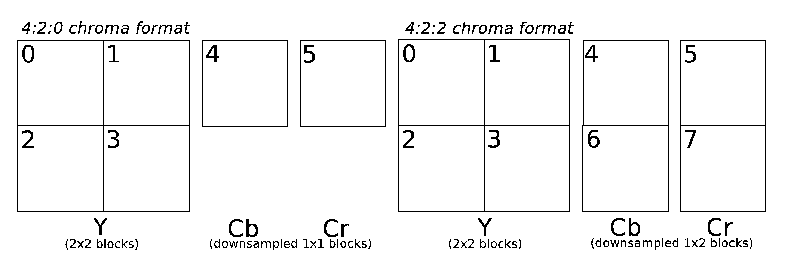
\epsfig{file=chroma_format.eps, width=2.5in}
    % \caption{4:2:0 and 4:2:2 chrominance formats showing macroblock ordering}
    % \label{fig:chroma-format}
   \end{center}
  }
  \end{minipage}
  \caption{Decoding stream to handle 4:2:0 and 4:2:2 chroma
    formats. Figures on right illustrate how macroblock orderings
    differ.}
  \label{fig:chroma}
\end{figure*}



